\documentclass[12pt, twocolumn]{article}
\usepackage{amsmath}
\usepackage{amsfonts}
\usepackage{graphicx}
\usepackage{mathtools}
\usepackage{fullpage}
\usepackage{float}
\usepackage{color, soul}

\begin{document}
\title{ 6.867 Term Project: \\ An Exploration of Deep Learning and \\ Convolutional Neural Nets for Image Classification\\ }
 \author{Kathryn Evans, Andres Hasfura and Remy Mock}
\maketitle

\section{ Introduction} 
Neural networks are a useful machine learning framework. Their primary benefit is that instead of specifying the basis functions relating input to output, the basis function is learned.  This is especially useful for when the optimal basis function is complicated or non-intuitive, such as in the case of images.  Such an approach is Artificial Neural Networks (ANN). 


Through this course, a simple singular layer artificial neural network was presented. However, much like the neural networks in the human brain visual system which provided the inspiration for artificial neural networks, the architecture used for machine learning neural networks can be more complicated and complex than a single hidden layer. The idea of utilizing many layers is known as deep learning.  Increasing layers, while drastically more parameters and computation,  allows for more complex input/output relationship and an ability to classify based on both information from low and high level features.

Deep learning, although not a recent idea, has recently exploded in popularity due to rise in labeled data and general purpose GPU programming and is revolutionizing very important subfields within artificial intelligence. Machine learning, machine vision, and natural language processing are examples of area in which the use of deep learning has produced large jumps in performance on difficult test sets. Deep nets are now being used anywhere from pedestrian detection for autonomous vehicles \cite{Szarvas2006}, to facial expression recognition \cite{Li2015} to classifying whether or not a selfie is good \cite{Karpathy}. 
	
Not only do deep nets contain more hidden layers but a multitude of different types of layers. Each layer type has different connectivity and objectives allowing for a greater richness of information. For use with images convolutional layers are especially beneficial for examining only the relevance of spatially nearby pixels in the context of determining features. Arrangements of convolutional layers as well as other types of layers leads to Convolutional Neural Networks (CNN). 

In this project, we want to explore the benefits of deep nets as well as convolutional neural networks for image classification.  Our first goal is to generalize the benefit on image classification performance of firstly, additional fully connected hidden layers and secondly, more complicated convolutional layers and architectures but utilizing software we build. Not only do we want to gain familiarity with concept and tools used in deep learning but we also hope to document generalities by applying these approaches to multiple image datasets. The generalities we hope to explore include the following: How does the number of layers affect the amount of training data needed? How does a specific type of layer affect accuracy  or computation time? 

Our second goal is to attempt to replicate results from Yann Lecun on the classification of the MNIST data sets for more complicated frameworks like LeNet \cite{LeCun1998}. For this we will use the professional deep learning library to get faster results and be able to quickly build extensive architectures. 

This paper is organized as follows. First we will introduce fully connected and convolutional neural networks with an emphasis on types of layers and implementation. In the approach section we will also describe the dataset, MNIST, as well as those networks we wish to replicate.  Then we will describe our results starting with  results from the simplest, 3 layer convolutional neural network and a similarly sized fully connected network to explore benefits and extract generalities about design and parameter choices to deepen our understanding and intuition behind the network. We will then introduce the professional libraries and the extended architectures see how close to the published results we can achieve on MNIST. Lastly we will summarize our findings and successes.

\section{Approach and Methodology}
	
In this project, we seek to implement a version of multilayer neural nets for supervised learning on specifically images. We plan on trying our implementations on the data , so that we do not have to worry about data generation and labeling and provide generalization about the neural net choices. Because we are specifically interested in applying our implementation to images we hope to see benefit of making the network out of convolution layers, where not all nodes are connected and we will compare this to a implementation with fully connected layers.

 We will then compare our rudimentary approach to a professional library for deep learning, specifically TensorFlow. Obviously the professional library will allow for better results and the interesting conclusions but building and implementing a simplified version will give a better understanding into how the neural network works. 

\subsection{Neural Network Basics}

In general, the idea of a neural network replaces the known basis functions with features, which are parametric functions of activations, learned from the input data in the first layer of learning, and then utilize a second layer to learn the relationship of the output data from those selected features.

\begin{equation}
a_j^{(1)}= \sum_{i=1}^N w_{ji}^{(1)} x_i+w_{j0}^{(1)}
\end{equation}
\begin{equation}
z_j= g(a_j)
\end{equation}

Where $g(x)$ is a nonlinear map of input to $(0,1)$, generally tanh or sigmoid, and $a_j$ is an activiation, which depends on the data, $x_i, \; i=\{1,...N\}$  and learned weights $w_ji^{(1)}$ and bias $w_0^{(1)}$. 

The second layer learns in a similar fashion and can be describe for $K$ output classes and M features in the  hidden layer  is thus 
\begin{equation}
a_k^{(2)}= \sum_{j=1}^M w_jk^{(2)} z_j+w_{k0}^{(2)}
\end{equation}
\begin{equation}
f_k= \tilde{g}(a_k^{(2)})
\end{equation}
 
Where $\tilde{g}(x)$ is the activation function, another nonlinear map, not necessarily the same as $g(x)$ and $f_k$ is really our prediction $h_k(x,w)$. H

\begin{figure}
\includegraphics[scale=.6]{simpleNN.png}

\caption{Visualization of a simple Neural Network with 1 hidden layer \cite{Bishop} . }
\label{fig:basicNN}
\end{figure}


We will consider the cross entropy cost function, 

\begin{equation}
\scriptsize
J(w)= \sum_{i=1}^N \sum_{k=1}^K -y^{(i)}_k \textrm{log}h_k(x^{(i)})- (1 -y^{(i)}_k) \textrm{log}(1 -h_k(x^{(i)}))
\end {equation}



As the network grows in size, the computational time becomes more and more of a constraint. So for all studied neural networks we will used Stochastic Gradient descent as opposed to batch methods in order to find the optimal weights for each layer. 
\begin{equation}
w^{(t+1)} = w^{(t)} + \eta_t \nabla_w J(w^{(t)})
\end{equation}

Where $\eta$ is  the learning rate and the choice of that parameter is to be chosen to optimize results for a particular model on a particular data set.


\subsubsection{Backpropagation}

To use stochastic gradient descent  on the neural net, the back prop algorithm is used, which moves from input to output layers in forward propagation to calculate activations and then from output to input for the backward propagation to calculate the gradients. 


\subsection{Multi-layer Neural Network}
For each fully connected layer forward propagation is straight forward, as you simply continue the formula for a single hidden layer and chain them together for more layers. 

For backwards propagation, the error for each fully connected layer, $l$ is computed from the error of its output layer, $l+1$  

\begin{equation}
\delta^{(l)}=((W^{(l)})^T \delta^{(l+1)}) \cdot f ^{\prime} (z^{(l)})
\end{equation}

and the following derivatives for weights and biases, 
\begin{equation}
\nabla_{W^{(l)}}J(W,b;x,y) = \delta^{(l+1)}(a^{(l)})^T
\end{equation}
\begin{equation}
\nabla_{b^{(l)}}J(W,b;x,y)= \delta^{(l+1)}
\end{equation}

\subsubsection{Implementation}
Using MATLAB, we have implemented the Multi-layer Neural Network. It is soft-coded so the hidden layers and number of hidden nodes per layer can easily be altered. The function created cells for the weights of each layers and initialized the weights randomly between -1 and 1.
\newline
A sigmoid function shown below is used as the activation function.

\begin{equation}
\tilde{g}(x)= g(x) = \frac{1}{ 1+e^{-x}}
\end{equation}

A stochastic gradient descent approach was used with a step size $\eta$ shown below.
\begin{equation}
\eta = \frac{ \alpha}{ (\textrm{epoch} + \beta)^\gamma}
\end{equation}

where $\beta \leq 100$, $\gamma >.5$ and epoch is the number of times the descent method has gone through the training set.  
\newline\newline

To prevent over-fitting we used a regularization parameter $\lambda$. 


\subsection{General Architecture of a Convolutional Neural Network}
As opposed to a simple neural network, a convolutional neural network is specifically designed to take advantage of the 2-d structure of an input image by considering only local connections and tied weights followed by some form of pooling which results in translation invariant features. Compared to regular neural nets,  CNNs  have many fewer parameters than networks of similar size and thus they are easier to train. 



\subsubsection{Convolutional Layer}
The idea of the CNN is to no longer have fully connected layers. In a CNN, the relationship between two nodes are described by a kernel, ie. the convolutional kernel. But instead of hard coding the filters, the filters used are learned by training. 

By sub-sampling the image and having learned features over smaller segments of the larger image. The feature detector learning from the subsection can then be applied anywhere in the remaining image. Specifically, we can take the learned subsection features and convolve them with the larger image there by transforming the 2-D images into a 3-D space. For a  $M * N $ size image, using $K$ filters that are $m * n$,  after convolution, there are  $ K * (M - m + 1) * (N - n + 1) $ sub images. Using this method, we decrease the size of each image, but at the same time we learn low level features. 


Generally, the process that occurs in a convolution layer can be described as for each image, $x_n$ for $n=1..N$ and for each filter $k=1...K$ in the convolution layer, $c$
\begin{equation}
a_{n,k}^{(c)}= x_n \ast w_k^{(c)} + b_k^{(c)}
\end{equation}
\begin{equation}
f_{n,k}= \tilde{g}(a_{n,k}^{(c)})
\end{equation}
 
 Where $\ast$ is the convolution operator. 
 
 The number of feature maps directly controls capacity and so that depends on the number of available examples and the complexity of the task. The challenge is then to identify the correct filter size in order to obtain reasonable features, given a particular dataset.

Also CNNs introduce the idea of tied weights, which mean that certain connections between one layer to the next are defined to be the same. The tied weights dramatically reduces the number of parameters needed to describe and set up the network compared to a fully connected network of similar size. This idea is shown in fig. \ref{fig:conv}.



\begin{figure}
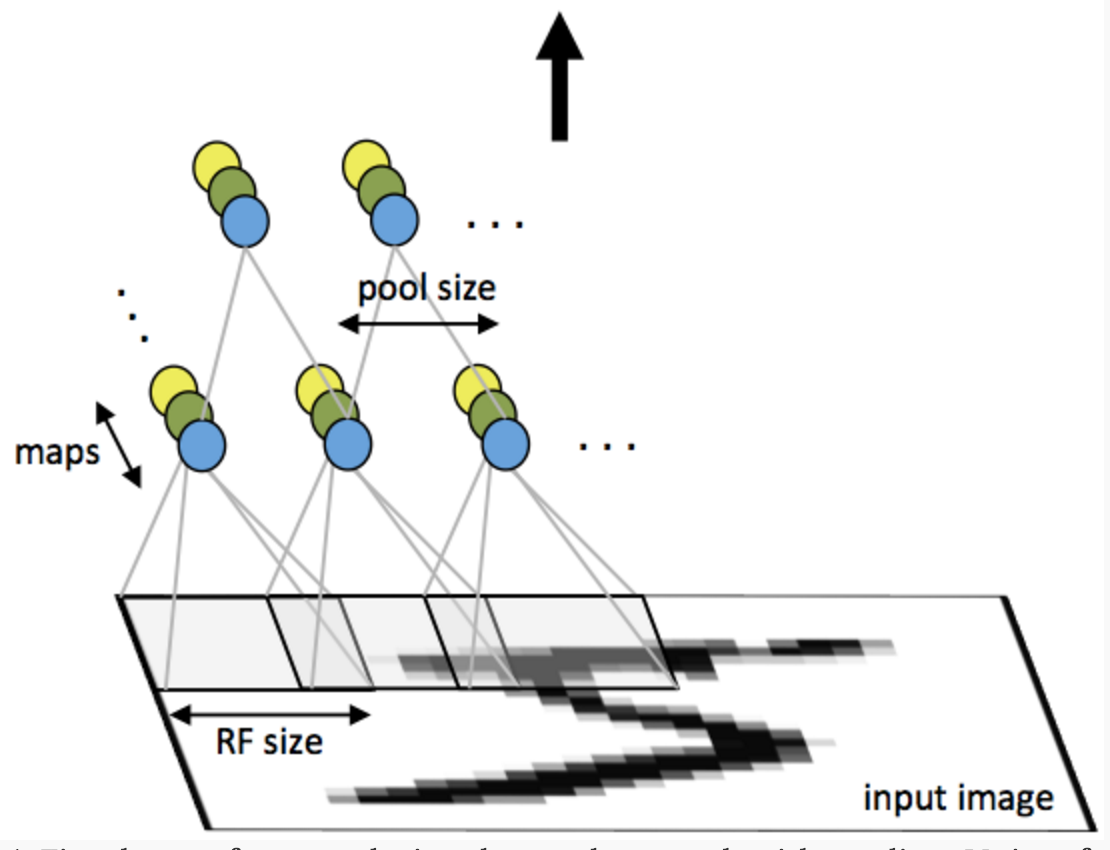
\includegraphics[scale=.4]{convgraphic.png}

\caption{Layer of a convolutional neural network with pooling. Nodes of the same color have tied weights and units of different color represent different filter maps \cite{StanfordTut}. }
\label{fig:conv}
\end{figure}


\subsubsection{Pooling Layer}
The features learned using convolution, are next used for classification. Previously with the fully connected neural network we utilized a softmax classifier, but this can be computationally challenging and expensive. Instead, pooling layers take advantage of a single parameter of these features, such as the mean, ( 'mean pooling') or max ( 'max pooling'), at  various regions in the image. Not only does this reduce the dimensionality of the result but can also help reduce over-fitting, a problem that is of serious concern for networks with increasing numbers of hidden nodes. 

The region to be pooled over is determined by the pooling dimensions. It again involves a convolution, this time between regions specified by the pooling dimensions and the results from the previous convolution layer. 

\subsubsection{Dropout}

Another common trick used in CNN is the inclusion of drop-out layers which help to decrease the likelihood of overfitting. It achieves this by essentially thinning out the number of hidden nodes by randomly dropping units during training.  A depiction of this effect is shown in Fig.~\ref{fig:dropout}. However, during test time all nodes are present. 
\begin{figure}
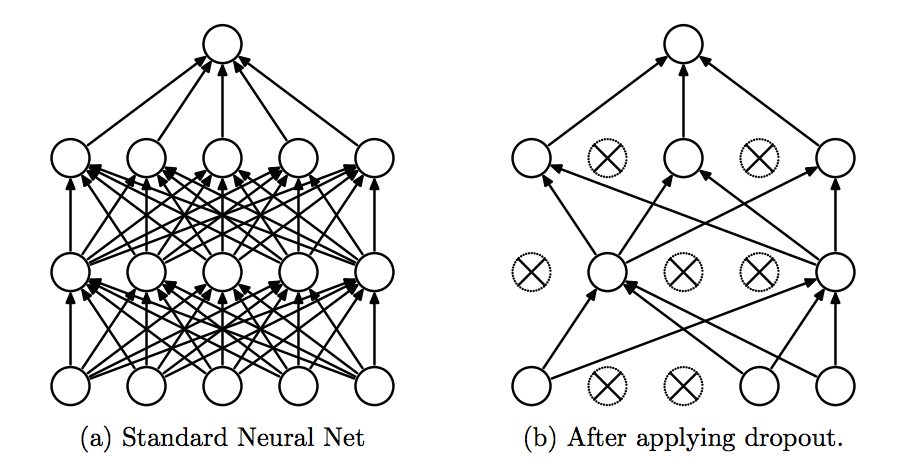
\includegraphics[scale=.52]{dropout.png}

\caption{Effect of dropout on a previously fully connected neural network. Dropped nodes are depicted as crossed out \cite{Dropout}. }
\label{fig:dropout}
\end{figure}

The simplest way to implement drop-out is to keep each node with probability, $p$, and otherwise discard it. The key benefit is that dropout is able to outperform regularization in neural networks for reducing overfitting \cite{Dropout}. Dropout also has the added benefit of being able to evaluate exponentially many different neural network architectures depending on which nodes are dropped.
 
\subsubsection{Re-LU}

Yet another problem with deep nets is that they are computationally expensive. One of the main tools to minimize this is a smart selection of the activation function, $g$. Specifically using a rectified linear unit, (Re-LU) as opposed to more traditional sigmoids or tanh, can be beneficial in increasing the efficiency of a neural network \cite{imagenet}. The Re-LU function is simple, 

\begin{equation}
g(x)= \textrm{max}(0,x)
\end{equation}

This function is not smooth but because the computation of $g$ is simply a comparison, it is generally much faster than smooth approximates. It also allows for sparse activation of the neural network, eliminating nodes with negative activations. 

\subsection{Backprop for CNN}
For fully connected layers  the derivative calculation remains the same. However,  error propagations are more complicated through the pooling and convolutional layers. 

For the pooling layer, the error must be up-sampled to propagate backwards
\begin{equation}
\delta^{(l)}_k=\textrm{upsample}((W^{(l)}_k)^T \delta^{(l+1)}_k) \cdot f^{\prime}(z^{(l)}_k)
\end{equation}


For mean pooling, with pool dimension, $p$, this is equivalent to 
\begin{equation}
delta^{(l)}= \frac{1}{\textrm{p}^2}  \textrm{kron}(\delta^{(l+1)}, \textrm{ones}(p))
\end{equation}
Where kron, is the Kroneckor Tensor Product.

Thus for the convolution layer, the derivatives can be calculated as follows.
\begin{equation}
\nabla_{W^{(l)}}J(W,b;x,y) = \sum_{i=1}^m (a^{(l)}_i) \ast \textrm{rot90}( \delta^{(l+1)}_k,2)
\end{equation}
\begin{equation}
\nabla_{b^{(l)}}J(W,b;x,y)= \sum_{a,b}(\delta^{(l+1)}_k)_{a,b}
\end{equation}


\subsection{Professional Libraries}

Since deep learning has become increasingly popular, optimized professional libraries that allow students, researchers and hobbyists to easily build complex deep nets are becoming easily accesible. There are many of these libraries, but we chose to adopt TensorFlow, the open source software from Google \cite{TensorFlowGH}. We especially like TensorFlow because it is python based, has abundant tutorials, is easy and intuitive to use. In addition, is uses an interface with Cuda for GPU processing to speed up results for image computations. \cite{TensorFlowWeb}. 



\subsection{Benchmarking with MNIST}


The MNIST is a well-known dataset of handwritten digits, 0-9, comprising 60,000 training examples and 10,000 test examples \cite{MNIST}  that can be used for image classification.  This data set arose from the U.S. Postal Service zip code database in order to help the scanning and transport of package to the right area. The images are all centered in 28 x 28.

\begin{figure}
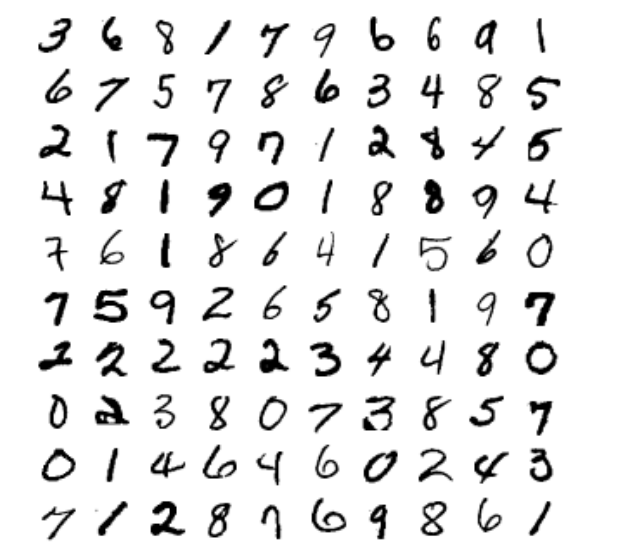
\includegraphics[scale=.8]{MNISTnos.png}
\label{fig:MNISTex}
\caption{Sample entries of the MNIST dataset \cite{LeCun1998}}
\end{figure}

Since the datatset has already been thoroughly explored on by many people including Yann LeCun \cite{LeCun1998}, it provides a good system to check our results.  Replication of the architecture of both the fully-connected and convolutional multi-layer neural nets provided in this paper is the first objective of our study. By comparing our results for different layers and types of layers to published and documented results, we can make sure our implementation is working correctly before taking on a more complicated dataset. 

\subsubsection{LeNets}
The CNN LeNet-1 architecture created by LeCun, consists of 5 layers, which are denoted by C1, S2, C3, S4, and F5.  The output of the first layer serves as
input to the next layer. C1 and C3 are convolution layers, and S2 and S4 are sub-sampling layers and the fifth layer is fully connected. \cite{LeCun89}

The CNN LeNet-4 architecture consists of 6 layers, which adds to LeNet-1 an additional hidden layer that is fully connected to its  input and output layers . \cite{LeCun95}

LeNet-5 architecture expands on this even further by adding an additional layer, with gaussian connections. More details on the architecture chosen, including filter size number and pooling dimension are shown in Fig. ~\ref{fig:LeNet5}

 \begin{figure*}
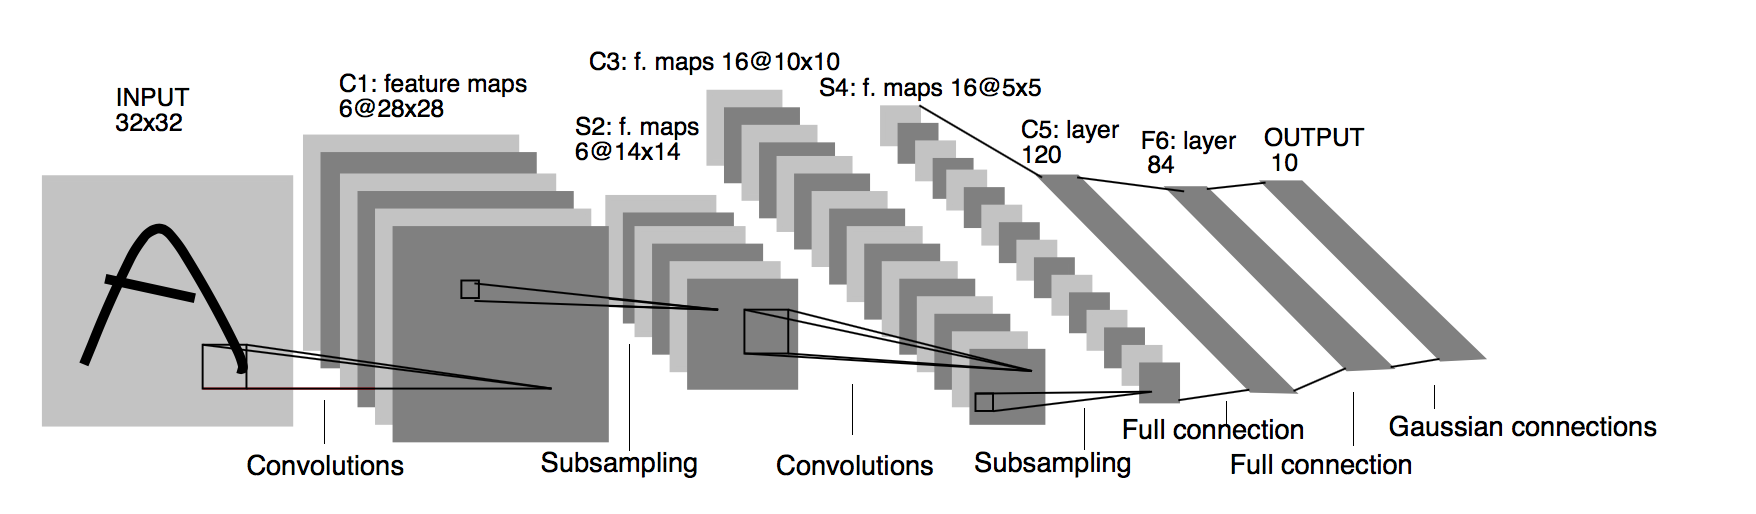
\includegraphics[scale=.6]{LeNet5.png}
\caption{Architecture for LeNet5 \cite{LeCun1998}}
\label{fig:LeNet5}
\end{figure*}


 We specifically chose to replicate the 2 and 3 layer fully connected neural nets as well as LeNet-1, -4 and -5 with no preprocessing or distortions. 


\section{Results}
We start by examining the effects of multiple layers and convolutional network layers to improve performance on MNIST using networks that we made. We will try to quantify accuracy gains versus computation time for different type of networks of relatively small size. To test bigger networks and to replicate LeCun's results we will transition to utilizing TensorFlow to classify MNIST images. 

\subsection{Multilayer NN}
\subsection{Simple CNN}
The first objective was to build the simplest CNN, comprising of one convolutional layer, one pooling layer and one fully connected layer and implement it on the full MNIST dataset to ensure that it works. We will examine individual design choices and parameters to gain intuition on how they impact the overall result. However, it is important to note than in all these cases we are not performing a full search over the parameter space so these are not necessarily true optima or fully generalizable statements. Rather they may be local maximas. In the sake of completely the project on time,  we will only concentrate on these small studies in the hope that we can glean useful information from them. 

\subsubsection{Efficiency}
iterations versus accuracy 

\subsubsection{Filter Sizes}

We decided to look at the effect of the filter size on the accuracy and computation time, while keeping all other parameters constant. Not surprisingly, increasing the filter size increases the computation time quadratically. However, the main takeaway is that after a certain threshold size, the accuracy seems not to be affected by the filter size. This idea is show in Fig.~\ref{fig:filtsize}. As long as the filter is bigger than 6x6 pixels, the net is able to achieve less than 4 $\%$ error on the testing data. For this architecture there is a optima at a filter size of 13 x 13 pixels, but this may just be an effect of other meta parameters. 
\begin{figure}
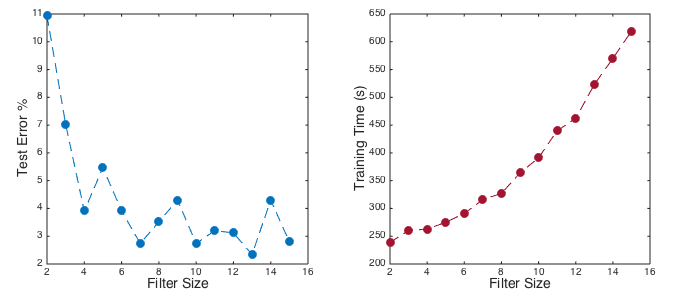
\includegraphics[scale=.35]{filtersize.png}
\caption{Effect of changing filter size on error and time}
\label{fig:filtsize}

\end{figure}


\subsubsection{Dropout Effect}
We also looked at changing the dropout rate, $p$ from .5 to 1, where $p=1$ is no dropout. Which the exception of one sharp peak, the computation time showed a logarithmic increase in computation time, making little difference at the high end of the range tested shown in Fig. ~\ref{fig:dropoutres}. It also show that high probabilities of dropout perform better than lower values and better than no dropout at all $p=1$. 
\begin{figure}
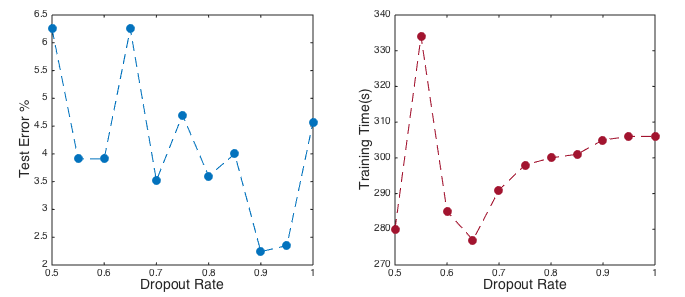
\includegraphics[scale=.35]{dropoutrate.png}
\caption{Effect of changing dropout rate on error and time}
\label{fig:dropoutres}
\end{figure}


\subsubsection{Pooling Method}
On this simple network we investigated the accuracy and computation time of utilizing mean versus max pooling. We expect computation time to be about the same since both operations are linear time. However we found that 

SMALL filter, MEDIUM BIG Filter,

\subsubsection{Pooling Size}

\subsubsection{Tanh versus ReLU}

The optimal combination for this simple three layer CNN was found to be with SIZE FILTERS, NUM NODES, DROPOUT, POOLING TYPE, and was found to have only a BLANK  BLANK error. 

For bigger CNNs we will turn to TensorFlow. 
\subsection{Replication of NNs and LeNets Results}





\begin{center}
\begin{table*}[t]
\begin{tabular} { |c | c | c | c | }
    \hline
    NN Type & LeCun Error  &  Our Error  & Tensor Flow Error \\ \hline
    2-layer NN, 300 hidden units, mean square error & 4.7 &  & \\ \hline
    2-layer NN, 1000 hidden units & 4.5 & & \\ \hline
    3-layer NN, 300+100 hidden units & 3.05 & &  \\ \hline
    3-layer NN, 500+150 hidden units & 2.95 & & \\ \hline
    3- layer CNN &  -- &  2.7 &  \\ \hline
    5 layer CNN  (LeNet-1) & 1.7 & -- & \\ \hline 
    6 layerCNN (LeNet-4) & 1.1& -- & \\ \hline 
    7 layer CNN (LeNet-5) &  0.95 &  -- &\\ \hline
\end{tabular}
\label{table: MNISTLeCun}
\caption{Comparison of Test Error results for multilayer ANN and CNN with published results \cite{LeCun1998}.}
\end{table*}
\end{center}



\section{Conclusions}

\subsection{Division of Labor}
Kathryn build the CNN. 
Andres led the implementation of TensorFlow and complex architectures.
Remy build multilayer neural nets. 

\subsection{Additional Insight: Multi-layer vs Single-layer}
According to the Universal Approximation theorem, in a compact and continuous data-set the two-layer neural network can perform as well as any multi-layer neural network given enough hidden nodes. Since in our tests the two layer network does not perform as well as the three layer network it is an interesting question to ask how many nodes we would need. Calculating the number of parameters of the two layer network with 1000 hidden nodes, 
\begin{equation}
\textrm{params} = 784*1000 + 1000* 10 = 794000
\end{equation}
\newline
and in the case of the 3 layer with 300 and 100 hidden nodes,
\begin{equation}
\textrm{params} = 784*300 + 300*100 + 100* 10 = 266200
\end{equation}
\newline
It is evident that the three-layer network outperforms the two-layer network with less parameters. 
\newline
\newline
In regards to time complexity, it is evident that the bottleneck of the function is back-propagation. Since the complexity back-propagation is related to the number of parameters it is also evident that the three-layer method has a lower time complexity.
\newline
\newline
It is clear from the two factors above that multi-layer is more efficient and is no surprise that deep learning is increasing in popularity.

\bibliographystyle{unsrt}
\bibliography{references}
\end{document}
